\vspace*{0cm}
\section{Introduction}
\label{sec:introduction}

Generative deep learning models have gained increasing interest in recent years due to their many applications and real-world use cases \cite{Goodfellow2014GenerativeNets, StyleGAN, BigGAN, VAE, VQVAE2, NVAE}. 
Given a dataset, their goal is to model a distribution that describes the processes of generating the data.
One family of generative models which allows both efficient sampling (i.e. generating new data) and exact density evaluation (i.e. determining the likelihood of a sample) is normalizing flows \cite{NormalizingFlowsFundamentals, NormalizingFlowsOriginalMathConcept}. 
Normalizing flows model distributions by applying a sequence of invertible transformations mapping the input distribution to a known base distribution such as a factorized Gaussian. 
In contrast to other common generative models like \acp{GAN} and \acp{VAE}, normalizing flows do not suffer from training issues like mode collapse or posterior collapse \cite{VAEPosteriorCollapse, StyleGAN, NormalizingFlowsOverview}. 
Successful applications of normalizing flows include image generation \cite{RealNVP, Glow, Flow++, IntegerNF}, audio generation \cite{FloWaveNet, Waveglow} and reinforcement learning \cite{NFReinforcementLearning1, NFReinforcementLearning2}.

The recent advances of normalizing flows concentrated on continuous distributions because the concept normalizing flows rely on is the rule of change of variables, a continuous transformation naturally working on continuous data.
However, many real-world applications involve discrete data, such as natural language, graphs and sets (see Figure~\ref{fig:introduction_categorical_applications}). 
Naturally, applying continuous flows on these discrete data points would lead to an undesired, degenerate solution where all probability mass is placed on only these discrete values, making the modeled distribution useless \cite{UriaContPeaks, Theis2015}. 
For the application on images, where close-by values are strongly related (i.e. a pixel value of 127 and 128 are almost visually indistinguishable), a common solution is to add a small amount of noise to each value for dequantization \cite{RealNVP, Flow++}.
Such dequantization techniques, however, cannot be as simply applied on nominal discrete data where the values represent categories with no intrinsic order. 
Treating these categories as integers for dequantization
biases the data to a non-existing order, and makes the modeling task significantly harder. 
Previous insights on learning the noise distribution in dequantization, called variational dequantization \cite{Flow++, EmielDequantization}, have underlined the great importance of a flexible representation of ordinal data in normalizing flows, and hence we suspect a similar impact for categorical data.

\begin{figure}[b!]
    \centering
    \begin{subfigure}{.3\textwidth}
        \centering
        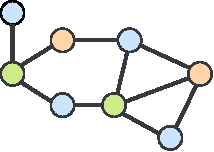
\includegraphics[height=2.5cm]{figures/intro_figures/graph_coloring.pdf}
        \caption{Combinatorial problems}
        \label{fig:introduction_applications_combinatorial_problems}
    \end{subfigure}
    \hfill
    \begin{subfigure}{.3\textwidth}
        \centering
        \vfill
        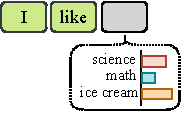
\includegraphics[height=2.5cm]{figures/intro_figures/language_modeling.pdf}
        \caption{Language modeling}
        \label{fig:introduction_applications_language_modeling}
    \end{subfigure}
    \hfill
    \begin{subfigure}{.3\textwidth}
        \centering
        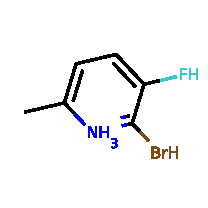
\includegraphics[height=2.5cm]{figures/intro_figures/zinc250k_tiny_981.pdf} %molecule_generation_rdkit.pdf}
        \caption{Molecule generation}
        \label{fig:introduction_applications_molecule_generation}
    \end{subfigure}
    \caption[Common applications and areas involving categorical distributions]{
    Common applications that involve categorical distributions include (a) combinatorial problems such as graph coloring, (b) language modeling and (c) use cases in biology and chemistry such as molecule generation. We will visit all three applications in experiments throughout this work.}
    \label{fig:introduction_categorical_applications}
\end{figure}

%%%%%%%%%%%%%%%%%%
%% Discrete NFs %%
%%%%%%%%%%%%%%%%%%
An alternative, which recently gained interested, is to apply normalizing flows directly on discrete distributions instead of continuous. 
This means that the input and the output distribution, as well as the intermediate steps in the flow model rely on discrete values. 
To implement this in a neural network, \citet{IntegerNF} proposed to use rounding operations on top of the continuous outputs of a neural flow to discretize it to the nearest integer. 
Another approach suggested by \citet{TranDiscreteFlows} operates on categorical distributions being suitable for non-ordinal data. 

However, while both have proven to work reasonably well in certain settings, there are considerable drawbacks with working directly on discrete space.
Firstly, discrete operations such as rounding or argmax are not differentiable, and thus cannot be used for backpropagation during training. 
Although solutions such as the straight-through estimator \cite{STEGradientEstimator} can approximate gradients for these operations, an experiment by \citet{IntegerNF} showed that a deep discrete flow obtains lower performance compared to a shallow flow.
This is because the gradient approximation accumulates bias with increasing depth, and destabilizes gradient-based optimization techniques \cite{IntegerNF, IDF++}.
Secondly, \citet{TranDiscreteFlows} discusses that their gradient approximation prevents them from scaling up to distributions with more than 200 categories.
Thus, such flows cannot be applied to large distributions like word-level language modeling.
Finally, discrete normalizing flows can only learn a permutation of its original input space, as the invertibility of the flow requires a one-to-one mapping from the input to the output \cite{SemiDiscreteNFSequence, IDF++, NormalizingFlowsOverview2}.
This limits the possible distributions it can model since with a uniform base distribution, any possible mapping learned by the flow will result in a uniform distribution.
Hence, discrete normalizing flows have to rely on powerful base distribution like autoregressive models as used in \cite{IntegerNF, TranDiscreteFlows}.

\begin{figure}[b!]
    \centering
    \begin{subfigure}{.48\textwidth}
        \centering
        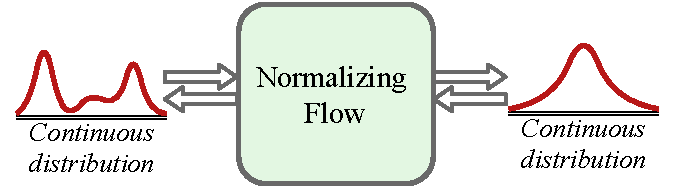
\includegraphics[width=\linewidth]{figures/intro_figures/GeneralNFs_Continuous_to_Continuous.pdf}
        \caption{Continuous Normalizing Flow}
        \label{fig:introduction_NFs_continuous_to_continuous}
    \end{subfigure}
    \hfill
    \begin{subfigure}{.48\textwidth}
        \centering
        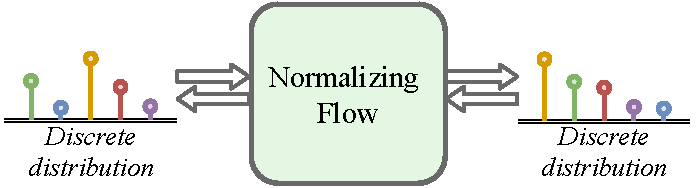
\includegraphics[width=\linewidth]{figures/intro_figures/GeneralNFs_Discrete_to_Discrete.pdf}
        \caption{Discrete Normalizing Flow}
        \label{fig:introduction_NFs_discrete_to_discrete}
    \end{subfigure}
    \begin{subfigure}{.48\textwidth}
        \centering
        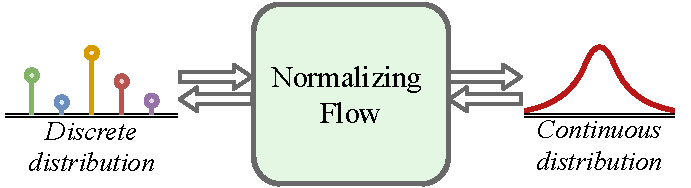
\includegraphics[width=\linewidth]{figures/intro_figures/GeneralNFs_Discrete_to_Continuous.pdf}
        \caption{Categorical Normalizing Flow}
        \label{fig:introduction_NFs_discrete_to_continuous}
    \end{subfigure}
    \caption[Comparison of Continuous, Discrete and Categorical Normalizing Flows]{
    Continuous normalizing flows are used to model a mapping between a complex, unknown continuous distribution to a base distribution like a Gaussian. 
    Discrete NFs map a discrete distribution to another by permuting its elements, being less flexible than a continuous flow.
    Our proposed approach, Categorical NF, also models discrete distributions, but stays with a continuous base distribution on the other side. This allows the usage of powerful continuous flows while operating on categorical data.}
    \label{fig:introduction_NFs_concept_semi_discrete}
\end{figure}

Meanwhile, continuous flows can learn much richer mappings between distributions. 
This allows them to model complex distributions using simple, factorized base distributions from which it can be efficiently sampled in parallel. 
Moreover, it has been theoretically shown that a flow on continuous data with sufficiently complex transformations can model a mapping between any two distributions \cite{NormalizingFlowsOriginalMathConcept, NormalizingFlowsOverview2}. 
Considering the issues of discrete normalizing flows, the question arises whether we can develop a method to apply powerful continuous flows on discrete, categorical input data.
Hence, in this work, we propose and investigate the framework of \emph{Categorical Normalizing Flows} which learn a mapping from a categorical distribution to a continuous base distribution while preserving a close-to exact likelihood estimate (see Figure~\ref{fig:introduction_NFs_discrete_to_continuous}). 




\subsection{Contributions}
\label{sec:introduction_contributions}

The first step in Categorical Normalizing Flows is to embed the discrete values into continuous space. 
Instead of pre-specifying non-overlapping volumes for each discrete value as done in dequantization, we propose to use variational inference as a toolkit to jointly optimize the mapping to continuous latent space and modeling the likelihood by a normalizing flow.
Previous work on combining variational inference with normalizing flows have mainly focused on improving the approximate posterior's flexibility \cite{InverseAutoregressiveFlows, NormalizingFlowsFundamentals, SylvesterNF}. 
Here, instead, we use variational inference to provide a continuous representation of the discrete data to a normalizing flow. 
Learning the continuous representation is crucial for categorical data as in contrast to integers, categories do not have an intrinsic order. On the contrary, there usually exist (hidden) relations between categories that may be beneficial to represent (i.e. similarity of word senses), and thus can be learned in Categorical Normalizing Flows.

To maintain a close-to exact likelihood estimate despite the introduced lower bound of the variational inference framework, the modeling of the categorical distribution needs to happen solely in the normalizing flow.
Thus, no information should be lost when mapping the data into continuous space.
We achieve this by limiting the encoding distributions to ones whose (approximate) posterior is independent over discrete variables. 
As a result, we obtain a learned partitioning of the latent space with an almost unique decoding, which is jointly learned with the model likelihood in continuous space.
We call this approach \emph{Categorical Normalizing Flows} and experiment with three different encoding distributions of increasing flexibility: (1) a mixture model where every category is represented by a logistic, (2) a model with additional flows applied to each category independently, and (3) a normalizing flow spanning across all variables, similar to variational dequantization.
Nonetheless, we find that in general a simple mixture model is sufficient for encoding categorical data well, and that increasing the complexity of the encoding distribution does not lead to a noticeable performance gain.

Categorical Normalizing Flows can be applied to any task involving categorical variables.
Examples, which we visit experimentally in this work, include words as categorical (one-hot vector) variables, sets and graphs~\cite{GraphOverview1, GraphOverview2}.
We put particular emphasis on graphs, as
current approaches are mostly autoregressive \cite{GraphRNNDeep, GraphAF, GraphRNN} and view graphs as sequences, although there exists no intrinsic order of the nodes. 
Normalizing flows, however, can perform generation in parallel making a definition of order unnecessary. 
By treating both nodes and edges as categorical variables, we employ our variational inference encoding and propose GraphCNF.
GraphCNF is a novel permutation-invariant normalizing flow on graph generation which assigns equal likelihood to any ordering of nodes. 
Meanwhile, GraphCNF encodes the node attributes, edge attributes and graph structure in three consecutive steps for efficiency.
As shown in the experiments on graph coloring and molecule generation, the improved encoding and flow architecture allows GraphCNF to outperform significantly both the autoregressive and parallel flow-based state-of-the-art.

Overall, our contributions are summarized as follows:
\begin{itemize}
	\item We propose Categorical Normalizing Flows, which apply a novel encoding method for categorical data in normalizing flows. 
	By using variational inference with a factorized posterior, we still support a close-to exact likelihood estimate and scale up to large number of categories.
	\item Building on the framework of Categorical Normalizing Flows, we propose GraphCNF, a permutation-invariant normalizing flow on graph generation.
	On molecule generation, GraphCNF sets a new state-of-the-art for flow-based methods, outperforming one-shot and autoregressive baselines. 
	\item We experiment with encoding distributions of increasing flexibility on various tasks including sets, language and graphs, and show that a simple mixture model is sufficient for modeling discrete, categorical distribution accurately. Moreover, we show that the encoding dimensionality also corresponds to the task's complexity underlining the importance of applying flexible, continuous flows on categorical data.
\end{itemize}


\subsection{Outline}
\label{sec:introduction_outline}
This thesis consists of six further sections. In Section~\ref{sec:background}, we review the fundamentals and common design choices of normalizing flows. 
The related work, including Discrete Normalizing Flows and combinations of \acp{VAE} and normalizing flows, is discussed in Section~\ref{sec:related_work}. 
Continuing in Section~\ref{sec:methodology}, we introduce the framework of Categorical Normalizing Flows in detail. Furthermore, we present GraphCNF, a permutation-invariant normalizing flow on graphs. 
Section~\ref{sec:experiments} discusses experiments on set modeling, graph coloring, molecule generation and language modeling that have been performed to evaluate and analyze the frameworks mentioned before. 
Finally, Section~\ref{sec:conclusion} concludes this thesis with a reflection of the results and suggestions for future work. 